\section{Gyan Sampada YT Channel}

This video is more about the introduction to magnetism, history, and also the basics of the hysteresis curve, and some basic information about the curie temperature, domains, domain-walls. 
\subsection*{V1. Ferromagnetism: Introduction and General Properties}
\addcontentsline{toc}{subsection}{1. Ferromagnetism: Introduction and General Properties}

\begin{enumerate}
    \item Ferro indicates the properties or presence of iron, originated from the latin word Ferrum - Iron.
    \item \textbf{Magnetism} - Physical phenomena that are mediated by magnetic field.
    \item There are two different shoruces of magnetic field, i. permanent magnet (ii.) electromagnet.
    \item Types of magnetic materials:
    \begin{enumerate}
        \item Ferromagnets
        \item Paramagnets
        \item Diamagnets
    \end{enumerate}
    \item \textbf{Ferromagnets:}
    \begin{enumerate}
        \item Strongly attracted by magnetic fields
        \item Ex: Fe, Co, Ni, alloys of steel
        \item First time ferromagnetism was observed in Load stones $(\mathrm{Fe_3O_4})$.
        \item The main characteristics of a ferromagnetism is \hl{\textbf{Spontaneous Magnetization}}. It is magnetization present prior to the application of an external field in the system. This magnetization is termed as spontaneous magnetization.   
        \item The spins in the ferromagnetic materials are equal and parallel to each other where each of them contribute to the total magnetic moment of the material. This is the tendency of the object to align with the applied magnetic field.
        \item It is analogous to ferro electricity. The only difference is that, if we have magnetic field, they will have electric field.
        \item Magnetism of any material would be non-linear if the external magnetic field is applied on the system. This phenomena traces the hysteresis loop. 
    \end{enumerate}\vspace{1cm}
    \item \textbf{Hysteresis Curve:}
    \begin{enumerate}
        \item Greek -> Hysteros -> Later -> Retardation in material's response with respect to applied field.
        \begin{figure}[h!]
            \centering
            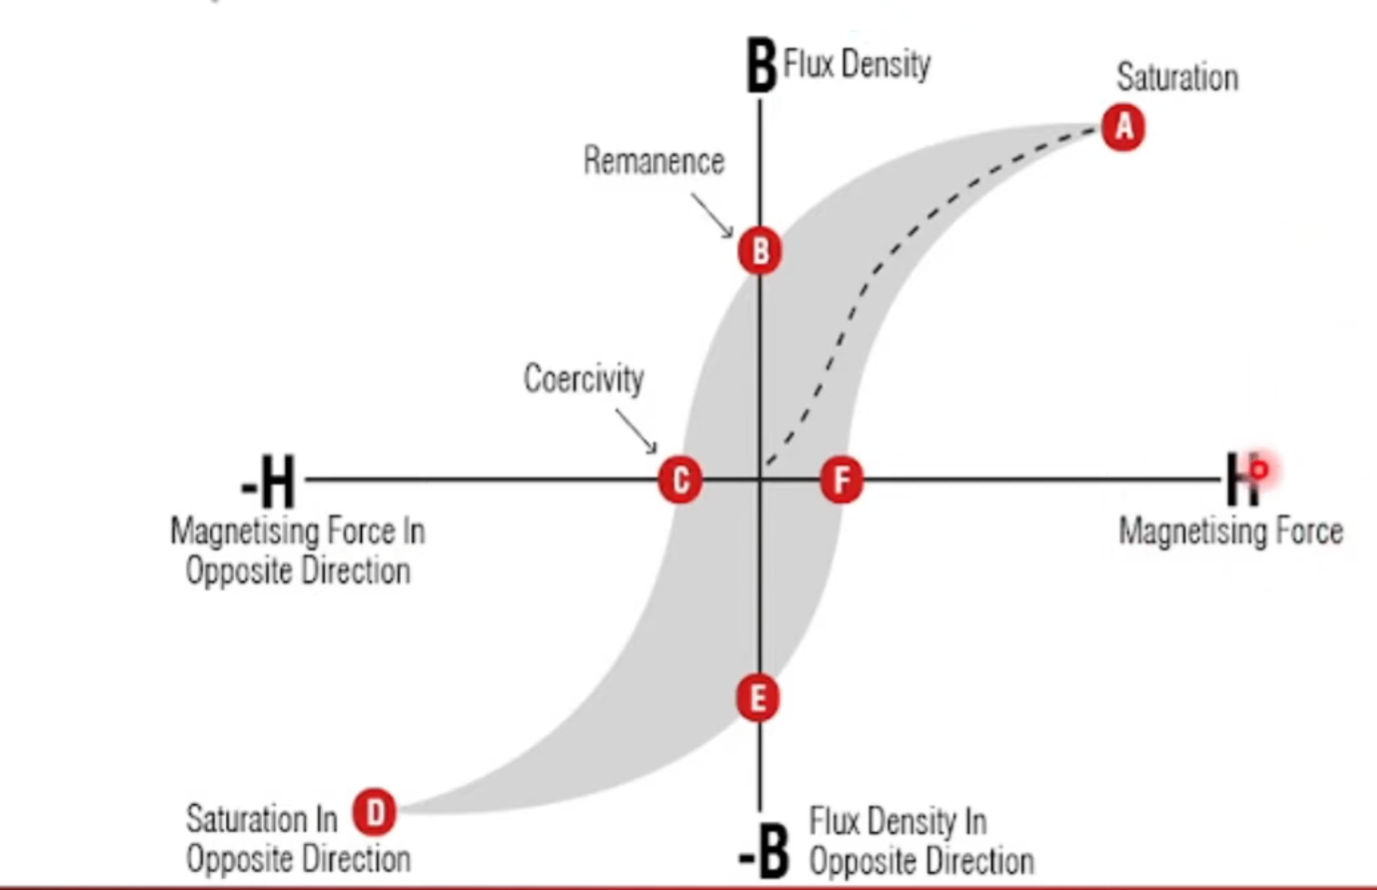
\includegraphics[width=0.85\linewidth]{Images/hysteresis_curve.png}
            \caption{Details of hysteresis curve.}
            \label{fig:hysteresis plot 1 }
        \end{figure}
        \item \underline{Step 1:} When the external field is applied in the $\mathrm{+ve}$ H direction, the spins/magnetic moment tries to align in the direction of the applied field. 
        \item \underline{Step 2:} Now if the external magnetic field is reduced, there remains some magnetization in the system. It does not trace back the same path and at 0 external field the magnetization is changed, this is termed as Remanence, and this is called Retentivity of the system.
        \item \underline{Step 3:} Further, to reduce the magnetization to its initial state, a negative external field is applied and at specific value the magnetization is reset and that point is termed as " Coercivity" and that field is called as coercive field.
        \item \underline{Step 4:} Again, when the magnetization is increased continuously in the negative direction, the magnetic moments/spin will orient in that direction and reaches saturation in the negative direction. 
    \end{enumerate}
    \item Spontaneous Magnetization disappears at $\mathrm{T_c}$ (\textbf{Ferromagnetic transition/Curie Temperature})
    \item Well above the transition temperature, material behaves like the paramagnetic material which is given by the Curie-Weiss Law,
    \begin{equation}
        \mathrm{T_c},\chi=\frac{C}{T-T_c}
        \label{eqn: curie-weiss law}
    \end{equation}
    \item Above $\mathrm{T_c}$ the magnetic moments are oriented randomly with net zero magnetization which is only in the case of paramagnetic materials.
    \item Made of large number of domains and each domain contains about $(10^9-10^{15})$. The direction might be different in different domains, but the direction in a particular domain would be the same. And the magnitude of the magnetic moment in the single domain is determined by the vector sum of the individual domains, schematically represented in figure \ref{fig:magnetic domains example}. And the boundaries which separates them is called \hl{domain-walls}. 
    \begin{figure}[h!]
        \centering
        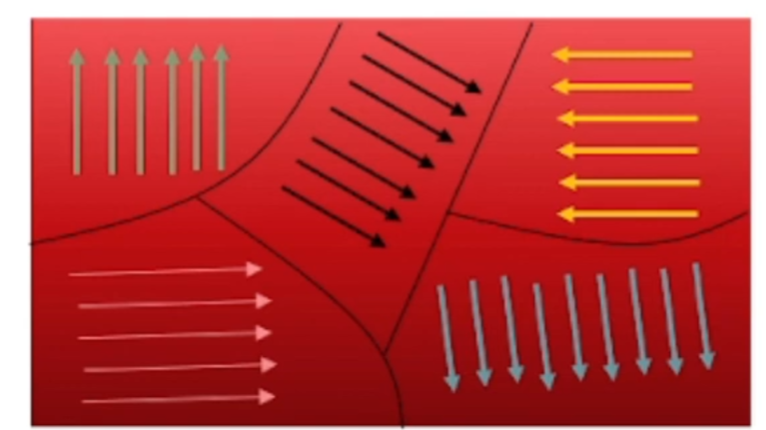
\includegraphics[width=0.75\linewidth]{Images/domains_example.png}
        \caption{A schematic representation of the magnetic domains in a ferromagnetic material.}
        \label{fig:magnetic domains example}
    \end{figure}
    \item Saturation magnetization (spontaneous magnetization in the case of temperature less than $T_c$) is increasing as the temperature decreases and maximum at $\mathrm{T=0} K$. This is also known as the normalized magnetization.
    \item Generally ferromagnetism appears in both metals and insulators.
\end{enumerate}